\documentclass[a4paper, 12pt]{article}

\usepackage{cmap}
\usepackage{mathtext} 
\usepackage[T2A]{fontenc}
\usepackage[utf8]{inputenc}
\usepackage[english,russian]{babel}	

\usepackage{amsfonts,amssymb,amsthm,mathtools}
\usepackage{amsmath}
\usepackage{icomma} 

\usepackage{graphicx} 
\graphicspath{{Picturies/}}
\usepackage{wrapfig}

\usepackage{array,tabularx,tabulary,booktabs}
\usepackage{longtable}
\usepackage{multirow}

\usepackage{caption}
\captionsetup{labelsep=period}

\renewcommand{\phi}{\varphi}
\newcommand{\eps}{\varepsilon}
\newcommand{\parag}[1]{\paragraph*{#1:}}
\newcommand{\mysec}[1]{\begin{center}\section*{#1}\end{center}}

\author{Радькин Кирилл Б01-005}
\title{3.2.3. Резонанс токов}
\date{13.09.21}

\graphicspath{{pictures/}}


\begin{document}

\maketitle

\parag {Цель работы} изучение параллельной цепи переменного тока, наблюдение резонанса токов.

\parag {В работе используются} лабораторный автотрансформатор (ЛАТР), разделительный понижающий трансформатор, емкость, дроссель с переменной индуктивностью, три амперметра, вольтметр, реостат, электронный осциллограф, омметр, мост переменного тока.
\\

В работе изучается параллельный контур, одна из ветвей которого содержит индуктивность $L$, другая емкость $C$. Через $r_L$ обозначено активное сопротивление катушки, которое включает в себя как чисто оммическое сопротивление витков катушки, так и сопротивление, связанное с потерями энергии при перемагничиваниии сердечника катушки. Активным сопротивлением емкостной ветви контура можно пренебречь, т.к. используемый в работе конденсатор обладает малыми потерями.
\\

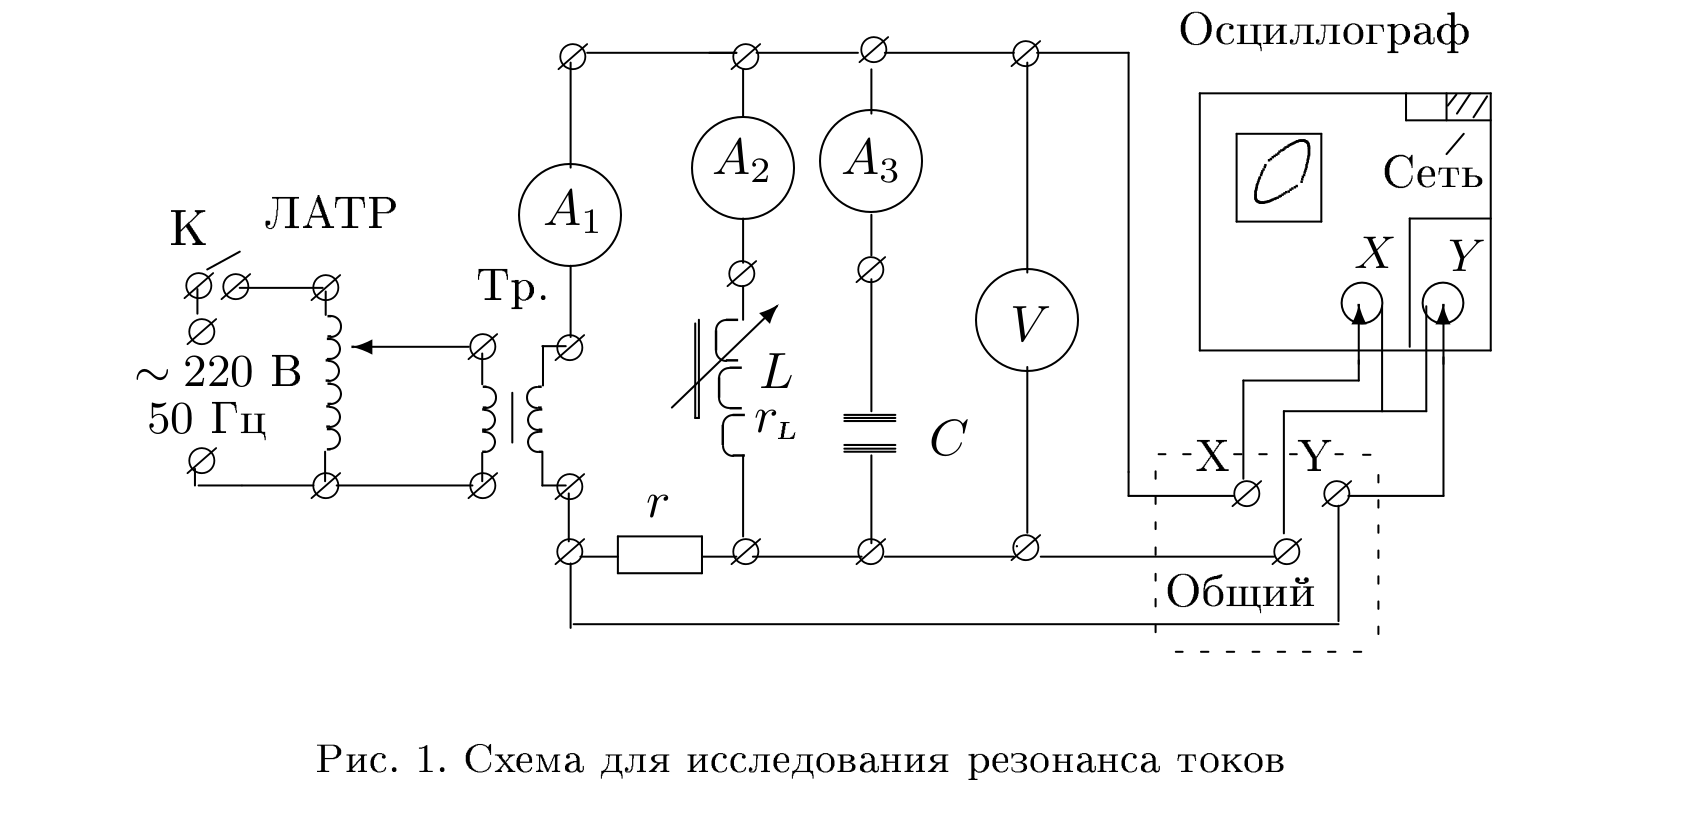
\includegraphics[scale=0.2]{ust.png}
\\

\parag {Экспериментальная установка} Схема экспериментальной установки приведена на рис. 1. Напряжение от сети ($220 В, 50 Гц$) с помощью ЛАТРа через понижающий трансформатор $Тр$ подается на параллельный контур, содержащий конденсатор ($C = 120 мкФ$) и катушку, индуктивность которой зависит от глубины погружения сердечника. Полный ток в цепи измеряется с помощью многопредельного амперметра $A_1$; для измерения токов в $L-$ и $C-$ветвях используются два одинаковых амперметра $A_2$ и $A_3$; напряжение на контуре контролируется электронным вольтметром $V$. Последовательно с контуром включен резистор $r$~---~реостат с полным сопротивлением $\simeq 100 Ом$.

Для наблюдения за сдвигом фаз между полным током и напряжением на контуре используется осциллограф. Сигнал, пропорциональный току, снимается с резистора $r$ и подается на вход $Y$ осциллографа. На вход $X$ подается напряжение непосредственно с конутра. При наличии сдвига фаз между этим напряжениями на экране виден эллипс, а при нулевом сдвиге фаз эллипс вырождается в прямую.

\mysec{Задание}

В работе предлагается снять при постоянном напряжении $U$ зависимости токов $I_L, I_C$ и полного тока $I$ от индуктивности катушки (глубины погружения сердечника), а также определить резонансные характеристики контура: полное сопротивление $R_{рез}$, добротность $Q$, активное сопротивление $r_L$ и индуктивность катушки $L_{рез}$.
\\
\begin{enumerate}
    \item Соберием схему согласно рис. 1. Для амперметров $A_2, A_3$ установим пределы измерения~---~$1$ А, для $A_1$~----~$0.5$ А. Полностью введем сердечник в катушку. По шкале на корпусе катушки это соответствует минимальному делению.
    
    \item Установим движок ЛАТРа в положение, соответствующее минимуму выходного напряжения (крайнее левое). Включим в сеть ЛАТР, катодный вольтметр и осциллограф.
    
    Плавным поворотом движка ЛАТРа установим напряжение на контуре (поэлектронному вольтметру) $V = 10 В$.

    \item Выдвигая сердечник дросселя и поддерживая с помощью ЛАТРа постоянное напряжение, определим диапазон перемещения сердечника, внутри которого общий ток $I$ в контуре не превышает $0.5 A$.
    
    Искомый диапазон: $3$~---~$11.5$ см. 

    \item Подобрав рабочий диапазон, снимем зависимости $I, I_L, I_C$ от координаты сердечника ($U = const$).
    
    \begin{tabular}{|c|c|c|c|}
        \hline
        $x, см$ & $I, \%$ от $0.5 A$ & $I_L, \%$ от $1 А$ & $I_C, \%$ от $1 А$ \\ \hline
        3 & 32 & 15 & 33 \\ \hline
        3.5 & 28 & 20 & 34 \\ \hline
        4 & 25 & 21 & 34 \\ \hline
        4.5 & 21 & 23 & 34 \\ \hline
        5 & 11 & 25 & 34 \\ \hline
        5.5 & 8 & 27 & 34 \\ \hline
        6 & 4 & 30 & 34 \\ \hline
        6.5 & 3 & 33 & 34 \\ \hline
        7 & 4 & 36 & 34 \\ \hline
        7.5 & 10 & 39 & 34 \\ \hline
        8 & 20 & 43 & 34 \\ \hline
        8.5 & 27 & 47 & 35 \\ \hline
        9 & 35 & 51 & 34 \\ \hline
        9.5 & 45 & 56 & 35 \\ \hline
        10 & 56 & 61 & 35 \\ \hline
        10.5 & 67 & 67 & 34 \\ \hline
        11 & 80 & 74 & 35 \\ \hline
        11.5 & 96 & 81 & 35 \\ \hline
    \end{tabular}
    \\\\
    Вблизи резонанса полный ток $I$ мал и по шкале $0.5 А$ измеряется неточно, но для наблюдения за общим ходом изменений это несущественно.

    Отметим, что эллипс вырождается в прямую при токе $I = 15 мА$.

    \item Вернием систему в положение резонанса (минимум полного тока в цепи) и, убрав напряжение до нуля, переключим амперметр $A_1$ на предел измерений $0.1 A$.
    
    \item Как можно точнее измерим резонансные значения трех токов и напряжение и убедимся с помощью осциллографа, что полное сопротивление цепи чисто активное.
    
    Оценим на месте добротность: $Q = 22$. $r_L = 4$ Ом.

    \item Убрав напряжение до нуля, отключим ЛАТР от сети и разберем схему.
\end{enumerate}

\newpage

\parag{Обработка результатов} 

\begin{enumerate}
    \item Построим на одном графике зависимости токов $I, I_L, I_C$ от положения сердечника: $I = f(x)$ ($x$~---~отсчет по шкале в мм).
    
    \item Рассчитаем добротность контура $Q$ через токи, и резонансное сопротивление $R_{рез}$~---~через полный ток и напряжение.
    
    $Q = \dfrac{I_{C, рез}}{I_{рез}} = \dfrac{I_{L, рез}}{I_{рез}} = 22$

    $R_{рез} = \dfrac{U_0}{I_{рез}} = 667$ Ом

    \item Рассчитаем $L_{рез}$ через емкость $C$ и частоту $\omega_0$ ($\nu_0 = 50$ Гц), а $r_L$~----~через емкость и добротность.
    
    $L_{рез} = \dfrac{1}{4 \cdot \pi^2 \cdot \nu_0^2 \cdot C} = 0.08$ Гн
    
    $r_L = \dfrac{1}{2 \cdot \pi \cdot \nu_0 \cdot C \cdot Q} = 1.2$ Ом

    \item Рассчитаем индуктивность $L_{рез}$ через $U$ и $I_{L, рез}$
    
    $L_{рез} = \dfrac{U_0}{2 \cdot \pi \cdot I_{L, рез}}$
\end{enumerate}

\end{document}
